\chapter{Proves i tests}
\label{cha:tests}
En aquest capítol descrivim les proves realitzades de la aplicació en diferents entorns. Els objectius de les proves es provar el rendiments amb mesures de temps, la robustesa i finalment s'explicaran les dificultats trobades.

\section{Prova en PC local}
Aquests proves han sigut realitzades en un SONY Vaio VGN-NW21EF amb la següent especificaci\'{o}:
\begin{itemize}
\item Ubuntu 10.4 32 bits
\item 4gb RAM
\item 2 processadors Pentium(R) Dual-Core CPU T4300  @ 2.10GHz
\end{itemize}
En aquest entorn s'ha instal.lat tots els components necessaris de la aplicaci\'{o} i amb la següent configuraci\'{o}:
\begin{itemize}
\item Ichnaea Software.
\item Gestor de cues RabbitMQ.
\item Sistema de cues per Ichnaea Software.
\item Servidor Web Apache.
\item Motor de dades MySQL.
\item SMTP deshabilitat. Les comunicacions es capturen mitjançant el \textit{profiler} de Symfony2.
\item Memoria cau deshabilitada.
\end{itemize}

\subsection*{Creaci\'{o} i administraci\'{o} d'usuaris}
S'han provat satisfactoriament totes les proves sense cap tipus de incid\`{e}ncia. Les funcionalitats son extensions del paquet FOSUserBundle, que cont\'{e} totes les funcionalitats provades per la comunitat.\cite{fosuserbundle}

\subsection*{Gesti\'{o} de matrius}

\subsubsection{Creaci\'{o} de matrius}
\label{cypruss}
Partim d'una matrius de dades reals proporcionada per Anicet Blanch anomenada \textit{Cypruss}. \'{E}s una matriu composta per 103 mostres de 27 variables(columnes). La matriu ha sigut proporciona en en format CSV.\\

La importaci\'{o} de matrius de dades \'{e}s una operaci\'{o} costosa ja que ha de llegir cadascun dels valors del fitxer. Seguidament el sistema renderitza la interficie de configuracions de matrius.\\

La creaci\'{o} del model de dades a partir d'un fitxer(lectura de totes les dades i modelat) triga de temps mig 1226ms. La renderitzaci\'{o} triga de temps mig 1066ms.\\

Si sumen ambdos temps surt un temps pro-mig d'importació i visualització de 2292ms. Es un temps excel·lent per una operació d'aquest tipus i amb tamany d'aquest fitxer.

\subsubsection{Esborrat de matrius}
Els esborrats de matrius han de esborrar totes les entitats dependents. En aquest cas ha d'esborrar tots els entrenaments i les prediccions creades a partir d'aquests entrenaments.\\

La prova \'{e}s d'un esborrat de matrius amb 4 entrenaments i dos prediccions ha trigat 1153ms. Es va comprovar correctament l'esborrat de les matrius, dels entrenaments i de les prediccions.

\subsubsection{Esborrat d'un entrenament}
Els esborrats de matrius han de esborrar totes les entitats dependents. En aquest cas ha d'esborrar totes les prediccions creades a partir de l'entrenament esborrat.\\

La prova d'un esborrat d'un entrenament amb dos prediccions triga 857ms. Es va comprovar correctament l'esborrat de l'entrenament i de les prediccions.

\subsubsection{Temps de resposta de les API JSON Restful}
Les llibreries de les interfícies enriquides son usades en les configuracions de matrius, tant de les normals com les de predicci\'{o}. Les proves s'han realitzat amb eines de mesures als navegadors: ''Firebug'' en Firefox i l'inspector natiu de Google Chrome. El temps m\'{i}nim calculat ha sigut 407ms i el m\'{a}xim 1050ms.\\

A la figura \fig{firebugAPI} es pot veure un diagrama de les peticions i els temps de resposta on a la columna ''Línia de temps'' es pot veure els temps trigats per peticions. Les peticions corresponents a demanar conjunts de fitxers i de salvar configuracions de columnes.
\begin{figure}[h]
  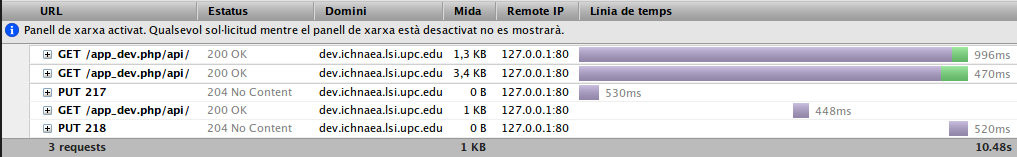
\includegraphics[scale=0.4]{img/test/firebugAPI.png}
  \caption{Línies de temps en proves de les funcions API Restful}
  \label{fig:firebugAPI}
\end{figure}


\subsubsection{Creaci\'{o} de matrius de predicci\'{o}}
\label{cypruss_test}
S'ha emprat una matriu de test proporcionada per fer prediccions de 19 mostres amb 27 variables(columnes). La importaci\'{o} de matrius de dades de prediccions \'{e}s una operaci\'{o} costosa ja que ha de llegir cadascun dels valors del fitxer. Seguidament el sistema renderitza la interficie de configuracions de matrius.\\

La creaci\'{o} del model de dades des d'un fitxer ha trigat 857ms i la renderitzaci\'{o} 855ms.

\subsubsection{Rendiment d'Ichnaea Software en aquest entorn}
Aquest projecte no consisteix en l'estudi de rendiment d'Ichnaea Software. Per\'{o} es interesant fer un estudi de temps en la realitzaci\'{o} dels procesos.

\paragraph{Entrenament de \textit{Cypruss}}
L'entrenament de la matriu \textit{Cypruss}(mirar \ref{cypruss}) ha tingut diferents mesures. S'han pres 3 mesures diferents: 1h 47min, 2h 15min i 1h 55min. Varia segons la carrega de la CPU i l'us de la memoria RAM. \'{E}s un proces que requereix una alta carrega de CPU.

\paragraph{Predicci\'{o} de \textit{Cypruss}}
La predicci\'{o} de la matriu de test(mirar \ref{cypruss_test}) ha tingut diferents mesure. S'han pres 3 messures diferents: 35min, 57min i 1h 5min, aproximadament. Varia segons la carrega de la CPU, ja que requereix una alta c\`{a}rrega de CPU.

\section{Prova en entorn distribuït}
Les proves en un entorn distribuït s'han realitzat en un m\'{a}quina virtual proporcionada per RdLab amb la següent especificaci\'{o}.

\begin{itemize}
\item 2 processadors QEMU Virtual CPU version 1.0 a2659Mhz
\item 2Gb RAM	
\item Linux version 3.2.0-30-generic
\end{itemize}
En aquest entorn s'ha instal.lat:
\begin{itemize}
\item Sense Ichnaea Software.
\item Sense gestor de cues RabbitMQ.
\item Sense sistema de cues per Ichnaea Software.
\item Servidor Web Apache.
\item Motor de dades MySQL en un altre servidor
\item SMTP habilitat.
\item Memoria cau habilitada.
\end{itemize}
No s'han pogut executar prediccions ni executar entrenaments.

\subsection{Creaci\'{o} i administraci\'{o} d'usuaris}
S'han provat satisfactoriament totes les proves sense cap tipus de incid\`{e}ncia. Les funcionalitats son extensions del paquet FOSUserBundle, que cont\'{e} totes les funcionalitats provades per la comunitat. 

\subsection{Gesti\'{o} de matrius}
\subsubsection{Creaci\'{o} de matrius}
Partim de la mateixa matriu de dades reals proporcionada. La importaci\'{o}(creaci\'{o} del model de dades a partir d'un fitxer) triga 1826ms i la renderitzaci\'{o} 1466ms sense haver passat per mem\'{o}ria cau. Despr\'{e}s de la segona execuci\'{o} la renderitzaci\'{o} tria 627ms.

\subsubsection{Temps de resposta de les API JSON Restful}
Les llibreries de les interficies enriquides son usades en les configuracions de matrius, tant de les normals com les de predicci\'{o}. El temps m\'{i}nim calculat ha sigut 216ms i el m\'{a}xim ha sigut 297ms.


\section{Dificultats trobades}
\label{sec:errorsKnown}
La realització de les proves han donat un conjunt de situacions que considero com a dificultats que s'han superades. 

\subsection*{Creació d'entrenaments parcials}
A l'hora de crear entrenaments existeix la possibilitat de crear entrenaments parcials, seleccionant les columnes que vols entrenar. Actualment Ichnaea Software utilitza un fitxer de configuració estàtic i esta esperant un conjunt de variables que si no es presenten dona un error de lectura del contingut de fitxers.\\

Actualment s'esta treballant en el projecte d'Ichnaea per solucionar aquest problema.

\subsection*{Flexibilitat en el model de dades}
La flexibilitat en el model de dades dona una quantitat de casuístiques elevades, sobretot en el la part de variables, conjunts de fitxers i components dels fitxers.\\

La possibilitat de compartir fitxers entre conjunts dona un conjunt de situacions que s'han hagut d'implementar les respostes per obtenir un sistema robust i que no doni errors de funcionament.

\subsection*{Herència de vistes en les interfícies de configuració de matrius}
Les interfícies de configuracions de matrius d'entrenaments i prediccions son molt semblants. Per tal de assolir la màxima coneguda en el mon de desenvolupament del \textit{software} de \textit{Don't repeat yourself}\cite{dontrepeat}, s'ha aprofitat la propietat de herència del motor de plantilles TWIG(seccio \ref{subsec:dependencies} a la p\`{a}gina \pageref{subsec:dependencies}) per abstreure el codi de les vistes de configuracions.\cite{herency}\\

El fet de no complir la màxima d'abans esmentada te conseqüències negatives com:
\begin{itemize}
\item repetició de codi
\item pobre mantenibilitat
\item risc mes elevat de repetir errors ja que no estan centralitzats
\end{itemize}


